\documentclass{beamer}
\usepackage{graphicx}
\usepackage{caption}
\usepackage{subcaption}
\usepackage{color}
\usepackage{listings}
\usepackage{verbatim}
\captionsetup{compatibility=false}
%\usepackage[italian]{babel}  

%% Se per qualsiasi motivo non riuscissi a compilare col tema Unipd,
%% basta commentare la riga qui sotto e si passa automaticamente al
%% tema beamer di default.
\usetheme{Unipd}

\lstdefinestyle{customc}{
  belowcaptionskip=1\baselineskip,
  breaklines=true,
  %frame=L,
  xleftmargin=\parindent,
  language=C,
  showstringspaces=false,
  basicstyle=\fontsize{7}{7}\selectfont\ttfamily,%\footnotesize\ttfamily,
  keywordstyle=\bfseries\color{green!40!black},
  commentstyle=\itshape\color{gray},
  identifierstyle=\color{blue!40!black},
  %stringstyle=\color{orange},
}
\lstset{escapechar=@,style=customc}

\title{Web Apps}
%\subtitle{da inserire}
\author{Diego Casella}
\date{\today}

\begin{document}

\maketitle

\begin{frame}{Contenuti} %Outline
\tableofcontents
\end{frame}

%% Introduzione
\section{Introduzione}
\begin{frame}{Introduzione}
Quando si vuole realizzare una applicazione che sia fruibile tramite web, slegata quindi da una installazione locale della stessa,
le soluzioni percorribili sono sostanzialmente due:
\begin{itemize}
\item creare uno ambiente desktop remoto, nel quale ogni utente possa disporre di una propria home separata e riservata dove poter eseguire l'applicazione;
\item eseguire l'applicazione direttamente nel browser;
\end{itemize}
Di seguito analizzeremo i vantaggi e gli svantaggi dei due approcci, confrontando le tecnologie pi\'u conosciute e diffuse.
\end{frame}

%
\section{Remote Desktop}
\begin{frame}{Remote Desktop}
Il Remote Desktop \'e una tecnologia attraverso la quale, come il nome stesso suggerisce, \'e possibile accedere ad una sessione
desktop situata in una macchina remota.
\newline
Si tratta di una tecnologia che si presta bene nella situazione in cui:
\begin{itemize}
\item l'applicazione che si vuole remotizzare sia gi\'a esistente, e dunque il tempo/costi di sviluppo per convertirla in una applicazione in browser siano troppo alti;
\item si abbia necessit\'a di accere al desktop remoto stesso, per eseguire operazioni di upload/download/modifica/creazione di
files, o operazioni di versioning;
\end{itemize}
\end{frame}


\begin{frame}{Remote Desktop - Realizzazione}
Il Remote Desktop viene realizzato attraverso una macchina remota, detta host, che contiene il software che si vuole rendere
fruibile a terze parti, e che \'e configurata ad hoc per poter gestire sessioni desktop multiple. Per poter fornire un grado di 
protezione superiore spesso l'host viene settato per accettare solo connessioni criptate, attraverso le quali poi viene effettuato
il tunnelling delle porte che interessano le effettive sessioni desktop.
\end{frame}


\begin{frame}{Remote Desktop - VNC}
Nel caso di sistema operativo GNU/Linux, uno dei programmi pi\'u diffusi per la creazione e gestione di desktop remoti \'e
chiamato VNC. Esso \'e suddiviso in due applicativi differenti:
\begin{itemize}
\item un server, eseguito in background, che inizializza e gestisce le varie sessioni desktop;
\item un client, sotto forma di applicazione standard, che consente di connettersi ad uno o pi\'u desktop remoti;
\end{itemize}
Dal momento che siamo interessati a capire come realizzare pi\'u sessioni desktop nel server remoto, ci focalizzeremo sul VNC
server.
\end{frame}


\begin{frame}{Remote Desktop - Setup VNC}
Per poter permettere ad un ipotetico utilizzatore \emph{Bob} di accedere alla sessione desktop remota, l'amministratore del
computer host deve:
\begin{itemize}
\item creare una nuova login e password per l'utente \emph{Bob};
\item fermare la sessione VNC esistente, tramite il comando \texttt{service vncserver stop};
\item editare il file di configurazione situato in \emph{/etc/sysconfig/vncservers} ;
\item inserire una password per VNC riferita all'utente \emph{Bob}, col comando \texttt{vncpasswd};
\item avviare una nuova sessione VNC, tramite il comando \texttt{service vncserver start};
\end{itemize}
\end{frame}


\begin{frame}{Remote Desktop - Setup VNC}
\begin{exampleblock}{Esempio di file vncservers}
{\small
VNCSERVERS="1:root 2:Fabio 3:Diego"
\newline
VNCSERVERARGS[1]="-geometry 1600x900  -localhost"
\newline
VNCSERVERARGS[2]="-geometry 640x480 -localhost"
\newline
VNCSERVERARGS[3]="-localhost"
}
\end{exampleblock}
La coppia \emph{(numero, utente)}, separata dal carattere '':'', indica in quale \emph{DISPLAY} indirizzare la sessione desktop
dell'utente associato. Inoltre tale numero, sommato al valore della porta 5900 usata di default da VNC, specifica attraverso quale
porta \'e possibile connettersi a tale sessione desktop.
\end{frame}


\begin{frame}{Remote Desktop - Setup VNC}
\begin{exampleblock}{Esempio di file vncservers}
{\small
VNCSERVERS="1:root 2:Fabio 3:Diego"
\newline
VNCSERVERARGS[1]="-geometry 1600x900  -localhost"
\newline
VNCSERVERARGS[2]="-geometry 640x480 -localhost"
\newline
VNCSERVERARGS[3]="-localhost"
}
\end{exampleblock}
L'opzione \emph{geometry} specifica la dimensione del desktop che verr\'a reso disponibile da VNC, tuttavia \'e un parametro che
non \'e obbligatorio mettere in quanto l'utente pu\'o comunque cambiarne la risoluzione a piacimento.
\end{frame}


\begin{frame}{Remote Desktop - Setup VNC}
\begin{exampleblock}{Esempio di file vncservers}
{\small
VNCSERVERS="1:root 2:Fabio 6:Bob"
\newline
VNCSERVERARGS[1]="-geometry 1600x900  -localhost"
\newline
VNCSERVERARGS[2]="-geometry 640x480 -localhost"
\newline
VNCSERVERARGS[6]="-localhost"
}
\end{exampleblock}
L'opzione  \emph{localhost} invece istruisce VNC di ignorare le connessioni provenienti dalle interfacce di rete, accettando solo
 quelle che sono originate dal server stesso. Quest'ultima opzione \'e fondamentale in quanto obbliga chi vuole connettersi al
 server VNC di instaurare per prima cosa una conessione protetta al server stesso, e poi fare un tunnelling della sessione desktop
 interessata.
\end{frame}


\begin{frame}{Remote Desktop - Connessione}
Ora che il setup del server \'e stato completato, vediamo come l'utente finale riesce a connettersi alla sua corrispettiva sessione
desktop remota.
\newline
Dal momento che, come detto in precedenza, il server accetta solo connessioni provenienti dal server stesso, occorre per prima cosa instaurare una connessione protetta al server stesso, dal quale effettuare poi il tunnelling della porta interessata.
\end{frame}


\begin{frame}{Remote Desktop - Connessione (2)}
Per poter realizzare tale connessione e tunnelling, sotto ambiente Windows \'e possibile utilizzare il client \emph{PuTTY} ,
 specificando il server al quale volersi connettere, la login per l'autenticazione, ed il port forwarding.

\begin{figure}
\centering
\begin{subfigure}{.5\textwidth}
  \centering
  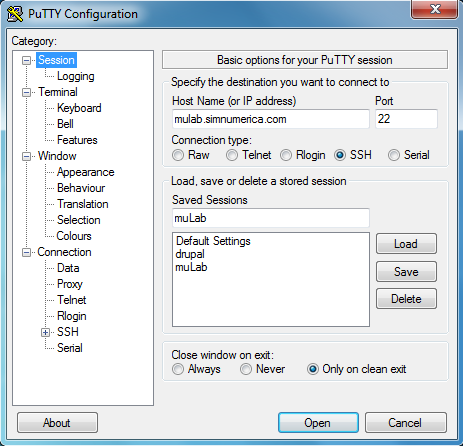
\includegraphics[scale=0.35]{images/putty_session_config.png}
\end{subfigure}%
\begin{subfigure}{.5\textwidth}
  \centering
  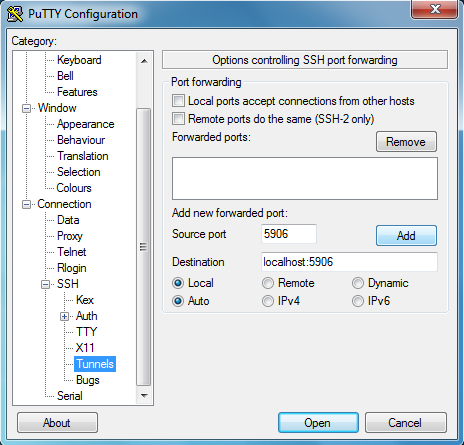
\includegraphics[scale=0.35]{images/putty_tunnelling_config.png}
\end{subfigure}
\caption{Esempio di configurazione di PuTTY}
\end{figure}

\end{frame}


\begin{frame}{Remote Desktop - Connessione (3)}
 In ambienti Unix invece \'e sufficiente aprire un terminale e digitare il comando
\newline
\texttt{ssh -L 5906:localhost:5906 -l Bob remote.host.com}
\newline
In entrambi i casi comunque, per poter procedere occorre inserire la password associata al desktop remoto di Bob .
\end{frame}


\begin{frame}{Remote Desktop - Connessione (4)}
Giunti a questo punto occorre utilizzare un client VNC, come ad esempio TightVNC, per potersi connettere al desktop remoto.
\begin{figure}
\centering
\begin{subfigure}{.5\textwidth}
  \centering
  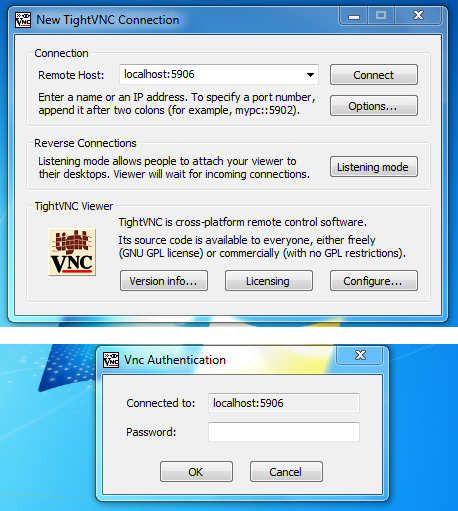
\includegraphics[scale=0.3]{images/tightvnc.png}
\end{subfigure}%
\begin{subfigure}{.5\textwidth}
  \centering
  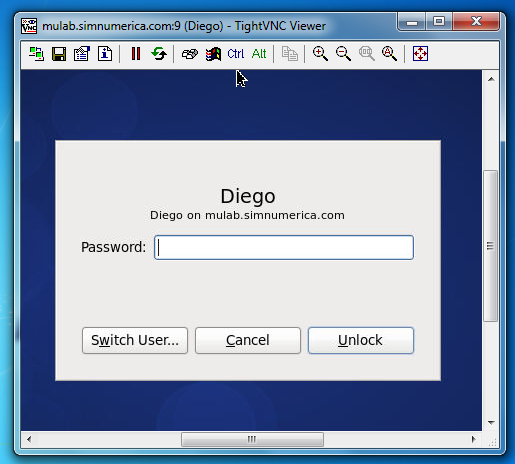
\includegraphics[scale=0.3]{images/tightvnc_rd.png}
\end{subfigure}
\caption{Esempio di connessione tramite TightVNC}
\end{figure}

\end{frame}

\begin{frame}{Remote Desktop - Pro}
\begin{itemize}
\item accesso al proprio spazio di lavoro da qualsiasi pc con una connessione internet;
\item l'utente finale non deve preoccuparsi di effettuare upgrade del software;
\item chiudendo VNC viewer, la sessione remota rimane persistente: si pu\'o dunque lanciare il software per eseguire calcoli
laboriosi, e monitorarlo di tanto in tanto;
\item possibilit\'a di utilizzare altri programmi presenti nell'host, come ad esempio toolchain di sviluppo, programmi di creazione di
report (openoffice), ecc... ;
\end{itemize}
\end{frame}

\begin{frame}{Remote Desktop - Contro}
\begin{itemize}
\item sono necessari l'uso di due software specifici per potersi connettere remotamente;
\item \'e inoltre necessario inserire 3 password, di cui almeno 2 obbligatorie;
\item se si esegue il logout nella sessione desktop remota, non \'e pi\'u possibile effettuare ulteriori login finch\'e l'
amministratore non riavvia il VNC server;
\item i tempi di risposta dipendono molto dalla qualit\'a della connessione a disposizone;
\end{itemize}
\end{frame}


\section{Remote Desktop - Fullscreen Application}
\begin{frame}{Remote Desktop - Fullscreen Application}
Un caso particolare del Remote Desktop \'e rappresentato dalla possibilt\'a di configurare ed utilizzare un window manager
 apposito, che faccia apparire solamente l'applicazione di interesse in modalit\'a fullscreen, disabilitando tutto ci\'o che riguarda
 taskbar, menu di sistema, analogamente a quanto accade negli ATM o nei terminali per comprare i bliglietti ferroviari.
\end{frame}



\begin{frame}{Remote Desktop - Fullscreen Application}
Se da un lato questa soluzione permette di impedire che l'utente esegua involontariamente un lougut dalla sua sessione, d'altro
lato gli impedisce di usare qualsiasi altro programma che possa tornargli utile per il suo workflow. Quindi sar\'a necessario che
questi tool vengano inclusi nell'applicativo principale, con notevole dispendio di tempo.
\end{frame}


\section{Web Application}
\begin{frame}{Web Application}
Un'altra tipologia di tecnologia per rendere disponibile un'applicazione da pi\'u locazioni differenti, senza dover obbligare l'utente
ad installare e configurare tale software, \'e rappresentata dalla categoria delle \emph{Web Application}.
Per Web Application si intende un gruppo molto esteso ed eterogeneo di applicazioni che, per funzionare, necessitano
semplicemente di un browser web.
\end{frame}


\subsection{Wicket}
\begin{frame}{Wicket}
Apache Wicket \'e la prima tipologia di framework per realizzare applicazioni web: si tratta di un framework scritto in Java per lo
sviluppo di siti web dinamici/web applications in cui la generazione delle pagine web viene demandata ad un servlet Java.
\end{frame}

\begin{frame}{Wicket (2)}
In Wicket viene usata una sintassi XHTML standard per creare i template delle pagine web. In essi, sono presenti dei tag con una
propriet\'a speciale denominata ''\emph{wicked:id}'': essa rappresenta la congiunzione fra l'elemento della pagina web, e il
componente Java ad esso associato, che diventa responsabile dell'output nella pagina web finale dello stesso.
 La pagina infine \'e semplicemente il componente di pi\'u alto livello, accoppiato ad esattamente un template XHTML, dal quale
dipartono i vari componenti figli.
\end{frame}

\begin{frame}{Wicket (3)}
\begin{exampleblock}{Esempio di Applicazione Wicket: HelloWorld.html}
{\small
$<$!DOCTYPE html PUBLIC "-//W3C//DTD XHTML 1.0 Transitional//EN" 
\newline
\hspace*{5 mm} "http://www.w3.org/TR/xhtml1/DTD/xhtml1-transitional.dtd"$>$
\newline
$<$html xmlns="http://www.w3.org/1999/xhtml" 
\newline
\hspace*{5 mm} xmlns:wicket="http://wicket.apache.org/dtds.data/wicket-xhtml1.3-strict.dtd" $>$
\newline
$<$body$>$
\newline
\hspace*{5 mm}$<$span wicket:id="message" id="message"$>$Errore nella visualizzazione del messaggio$<$/span$>$
\newline
$<$/body$>$
\newline
$<$/html$>$
}
\end{exampleblock}
\end{frame}

\begin{frame}{Wicket (4)}
\begin{exampleblock}{Esempio di Applicazione Wicket: HelloWorld.java}
{\small
package org.test.wicket;
\newline
import org.apache.wicket.markup.html.WebPage;
\newline
import org.apache.wicket.markup.html.basic.Label;
\newline
public class HelloWorld extends WebPage \{
\newline
\hspace*{5 mm}public HelloWorld() \{
\newline
\hspace*{10 mm} add(new Label("message", "Hello World!"));
\newline
\hspace*{5 mm}\}
\newline
\}
\newline
}
\end{exampleblock}
\end{frame}

\begin{frame}{Wicket - Pro}
\begin{itemize}
\item netta separazione fra core e presentazione;
\item uso di linguaggio di alto livello per realizzare pagine web (PHP \'e pi\'u ostico);
\item possibilit\'a di ridisegnare l'interfaccia senza toccare la logica di controllo;
\item il codice risiede tutto nel web server;
\end{itemize}
\end{frame}

\begin{frame}{Wicket - Contro}
\begin{itemize}
\item sintassi elaborata per realizzare anche semplici layout di elementi;
\item il server deve incaricarsi di gestire le sessioni utente, a differenza dei Remote Desktop;
\item tutte le utility presenti in una sessione desktop devono essere reimplementate nel software;
\item se il servlet Java \'e sotto carico di lavoro elevato o crasha, tutti gli utenti ne risentono;
\end{itemize}
\end{frame}

\subsection{Java Applet}
\begin{frame}{Java Applet}
Un'altra tecnologia per usufruire di applicativi web tramite broswer \'e rappresentata dalle Applet Java, ovvero bytecode Java
che viene caricato dal browser web ed interpretato non appena l'utente visita la pagina contenente tale applet.
\newline
Sostanzialmente, l'entry point \'e una istanza della classe JApplet (o sue sottoclassi), che viene eseguita dal browser stesso.
\end{frame}

\begin{frame}{Java Applet}
\begin{exampleblock}{Esempio di Applicazione Wicket: HelloWorld.java}
{\small
package org.test.japplet;
\newline
import javax.swing.JApplet;
\newline
import javax.swing.JLabel;
\newline
public class HelloWorld extends JApplet \{
\newline
\hspace*{5 mm}public HelloWorld() \{
\newline
\hspace*{10 mm} add(new JLabel("Hello World!"));
\newline
\hspace*{5 mm}\}
\newline
\}
\newline
}
\end{exampleblock}
\end{frame}

\begin{frame}{Java Applet - Pro}
\begin{itemize}
\item uso di linguaggio di alto livello per realizzare una applicazione web complessa;
\item sgrava il server dall'onere delle computazioni, che vengono eseguite nel browser dell'utente;
\end{itemize}
\end{frame}

\begin{frame}{Java Applet - Contro}
\begin{itemize}
\item il bytecode di ogni singola classe viene salvato nella cache del browser per essere eseguito, quindi applicazioni complesse
richiederanno pi\'u tempo per l'avvio;
\item non \'e possibile gestire le sessioni utente, a meno che non si utlizzi un servlet di appoggio (gestendone quindi la
comunicazione, oltre al fatto che tale servlet deve gestire ogni utente);
\item tutte le utility presenti in una sessione desktop devono essere reimplementate nel software;
\item le sandbox dei browser limitano le funzionalit\'a solitamente presenti (lettura/scrittura su fiel ad esempio, memoria 
disponibile);
\end{itemize}
\end{frame}

\subsection{Java Web Start}
\begin{frame}{Java Web Start}
Java Web Start \'e un altro framework per la creazione di Web Apps, che differisce leggermente dai due framework visti in
precedenza. Java si promuove come linguaggio ''\emph{write once, run everywhere}'' ma il problema \'e che l'installazione 
dell'applicazione, con annesse dipendenze ed upgrade dell'applicazione stessa, risulta difficile da gestire per l'utente medio.
\end{frame}

\begin{frame}{Java Web Start (2)}
Per questa ragione,Sun ha creato il Java Web Start: l'utente finale deve solo installare tale framework una volta e, ad ogni
utilizzo di un applicativo basato su Java Web Start, il framework stesso si occupa di tenerlo costantemente aggiornato, senza
 ulteriori interventi esterni.
\end{frame}

\begin{frame}{Java Web Start (3)}
L'applicativo Web Start viene scaricato nel computer quando l'utente, provvisto della runtime Web Start, clicca su un particolare
link che la runtime stessa identifica. Si avvia cos\'i il processo di download dell'applicazione e dei componenti necessari al 
funzionamento della stessa; da quel punto in poi, l'app sar\'a disponibile direttamente dal pc dell'utente senza l'utilizzo di un
browser come intermediario.
\end{frame}

\begin{frame}{Java Web Start - Pro}
\begin{itemize}
\item uso di linguaggio di alto livello per realizzare una applicazione web complessa;
\item sgrava il server dall'onere delle computazioni, che vengono eseguite nel pc dell'utente;
\item intero applicativo disponibile nel computer dell'utente;
\item funzionamento anche in assenza di connessione ad internet;
\end{itemize}
\end{frame}

\begin{frame}{Java Web Start - Contro}
\begin{itemize}
\item intero applicativo disponibile nel computer dell'utente;
\end{itemize}
\end{frame}

\section{Q\&A}
\begin{frame}{Q\&A}
\end{frame}

\end{document}
